
In case $1$ we see $\sigma = \sigma'$ and $k=m, l=n$ so we reduce to:
\begin{align*}
\bra{g}\sum_k c_{k}^\dagger \psi_{k}^\ast(\x) \sum_{l} c_{l}^\dagger \psi_{l,}^\ast (\x') \sum_k c_{k} \psi_{k}(\x') \sum_l c_{l} \psi_{l}(\x) \ket{g} \\
-\bra{g}\sum_k c_{k}^\dagger \psi_{k}^\ast(\x)  \sum_k c_{k} \psi_{k}(\x') \sum_{l} c_{l}^\dagger \psi_{l}^\ast (\x') \sum_l c_{l} \psi_{l}(\x) \ket{g} \\
-\bra{g}\sum_k c_{k}^\dagger \psi_{k}^\ast(\x) c_{k} \psi_{k}(\x') \sum_{l} c_{l}^\dagger \psi_{l}^\ast (\x') c_{l} \psi_{l}(\x) \ket{g} \\
-\bra{g}\sum_k c_{k}^\dagger c_{k} \psi_{k}^\ast(\x) \psi_{k}(\x') \sum_{l} c_{l}^\dagger  c_{l}\psi_{l}^\ast (\x') \psi_{l}(\x) \ket{g} \\
-\bra{g}\sum_k c_{k}^\dagger c_{k} \frac{1}{\sqrt{\V}} e^{i\vec{k}\cdot\x} \frac{1}{\sqrt{\V}}e^{-i\vec{k}\cdot\x'} \sum_{l} c_{l}^\dagger  c_{l} \frac{1}{\sqrt{\V}}e^{i\vec{l}\cdot\x'} \frac{1}{\sqrt{\V}}e^{-i\vec{l}\cdot\x}\ket{g} \\
\frac{-1}{\V^2}\bra{g}\sum_k c_{k}^\dagger c_{k} e^{i\vec{k}\cdot(\x-\x')} \sum_{l} c_{l}^\dagger  c_{l} e^{i\vec{l}\cdot(\x'-\x)} \ket{g} \\
-\frac{1}{\V}\sum_k e^{i\vec{k}\cdot(\x-\x')} \bra{g} c_{k}^\dagger c_{k} \ket{g} \frac{1}{\V} \sum_l e^{i\vec{l}\cdot(\x'-\x)} \bra{g} c_{l}^\dagger  c_{l} \ket{g} \\
-9\left(\frac{N}{2\V}\right)^2 \left( \frac{\sin(k_Fr) - k_Fr \cos(k_Fr)}{(k_Fr)^3}\right)^2
\end{align*}

In case $2$ we see $k=n, l=m$ so we reduce to:
\begin{align*}
\bra{g}\sum_k c_{k,\sigma}^\dagger \psi_{k,\sigma}^\ast(\x) \sum_{l} c_{l,\sigma'}^\dagger \psi_{l,\sigma'}^\ast (\x') \sum_l c_{l,\sigma'} \psi_{l,\sigma'}(\x') \sum_k c_{k,\sigma} \psi_{k,\sigma}(\x) \ket{g} \\
+\bra{g}\sum_k c_{k,\sigma}^\dagger \psi_{k,\sigma}^\ast(\x) \sum_k c_{k,\sigma} \psi_{k,\sigma}(\x) \sum_{l} c_{l,\sigma'}^\dagger \psi_{l,\sigma'}^\ast (\x') \sum_l c_{l,\sigma'} \psi_{l,\sigma'}(\x')  \ket{g} \\
\frac{1}{\V^2} \bra{g} \sum_k c_{k,\sigma}^\dagger c_{k,\sigma} \sum_l c_{l,\sigma'}^\dagger c_{l,\sigma'} \ket{g} \\
\left(\frac{N}{2\V}\right)^2
\end{align*}

Thus combining the final pieces:
\begin{align*}
\left(\frac{N}{2\V}\right)^2 -9\delta_{\sigma\sigma'}\left(\frac{N}{2\V}\right)^2 \left( \frac{\sin(k_Fr) - k_Fr \cos(k_Fr)}{(k_Fr)^3}\right)^2 = \left(\frac{N}{2\V}\right)^2 g_{\sigma\sigma'}(\x-\x') \\
1 -9\delta_{\sigma\sigma'} \left( \frac{\sin(k_Fr) - k_Fr \cos(k_Fr)}{(k_Fr)^3}\right)^2 =  g_{\sigma\sigma'}(\x-\x')
\end{align*}

And we see for $\sigma \neq \sigma'$ the density $g_{\sigma\sigma'}=1$.
For $\sigma = \sigma'$ the density looks as follows:

\begin{figure}[H]
\centering
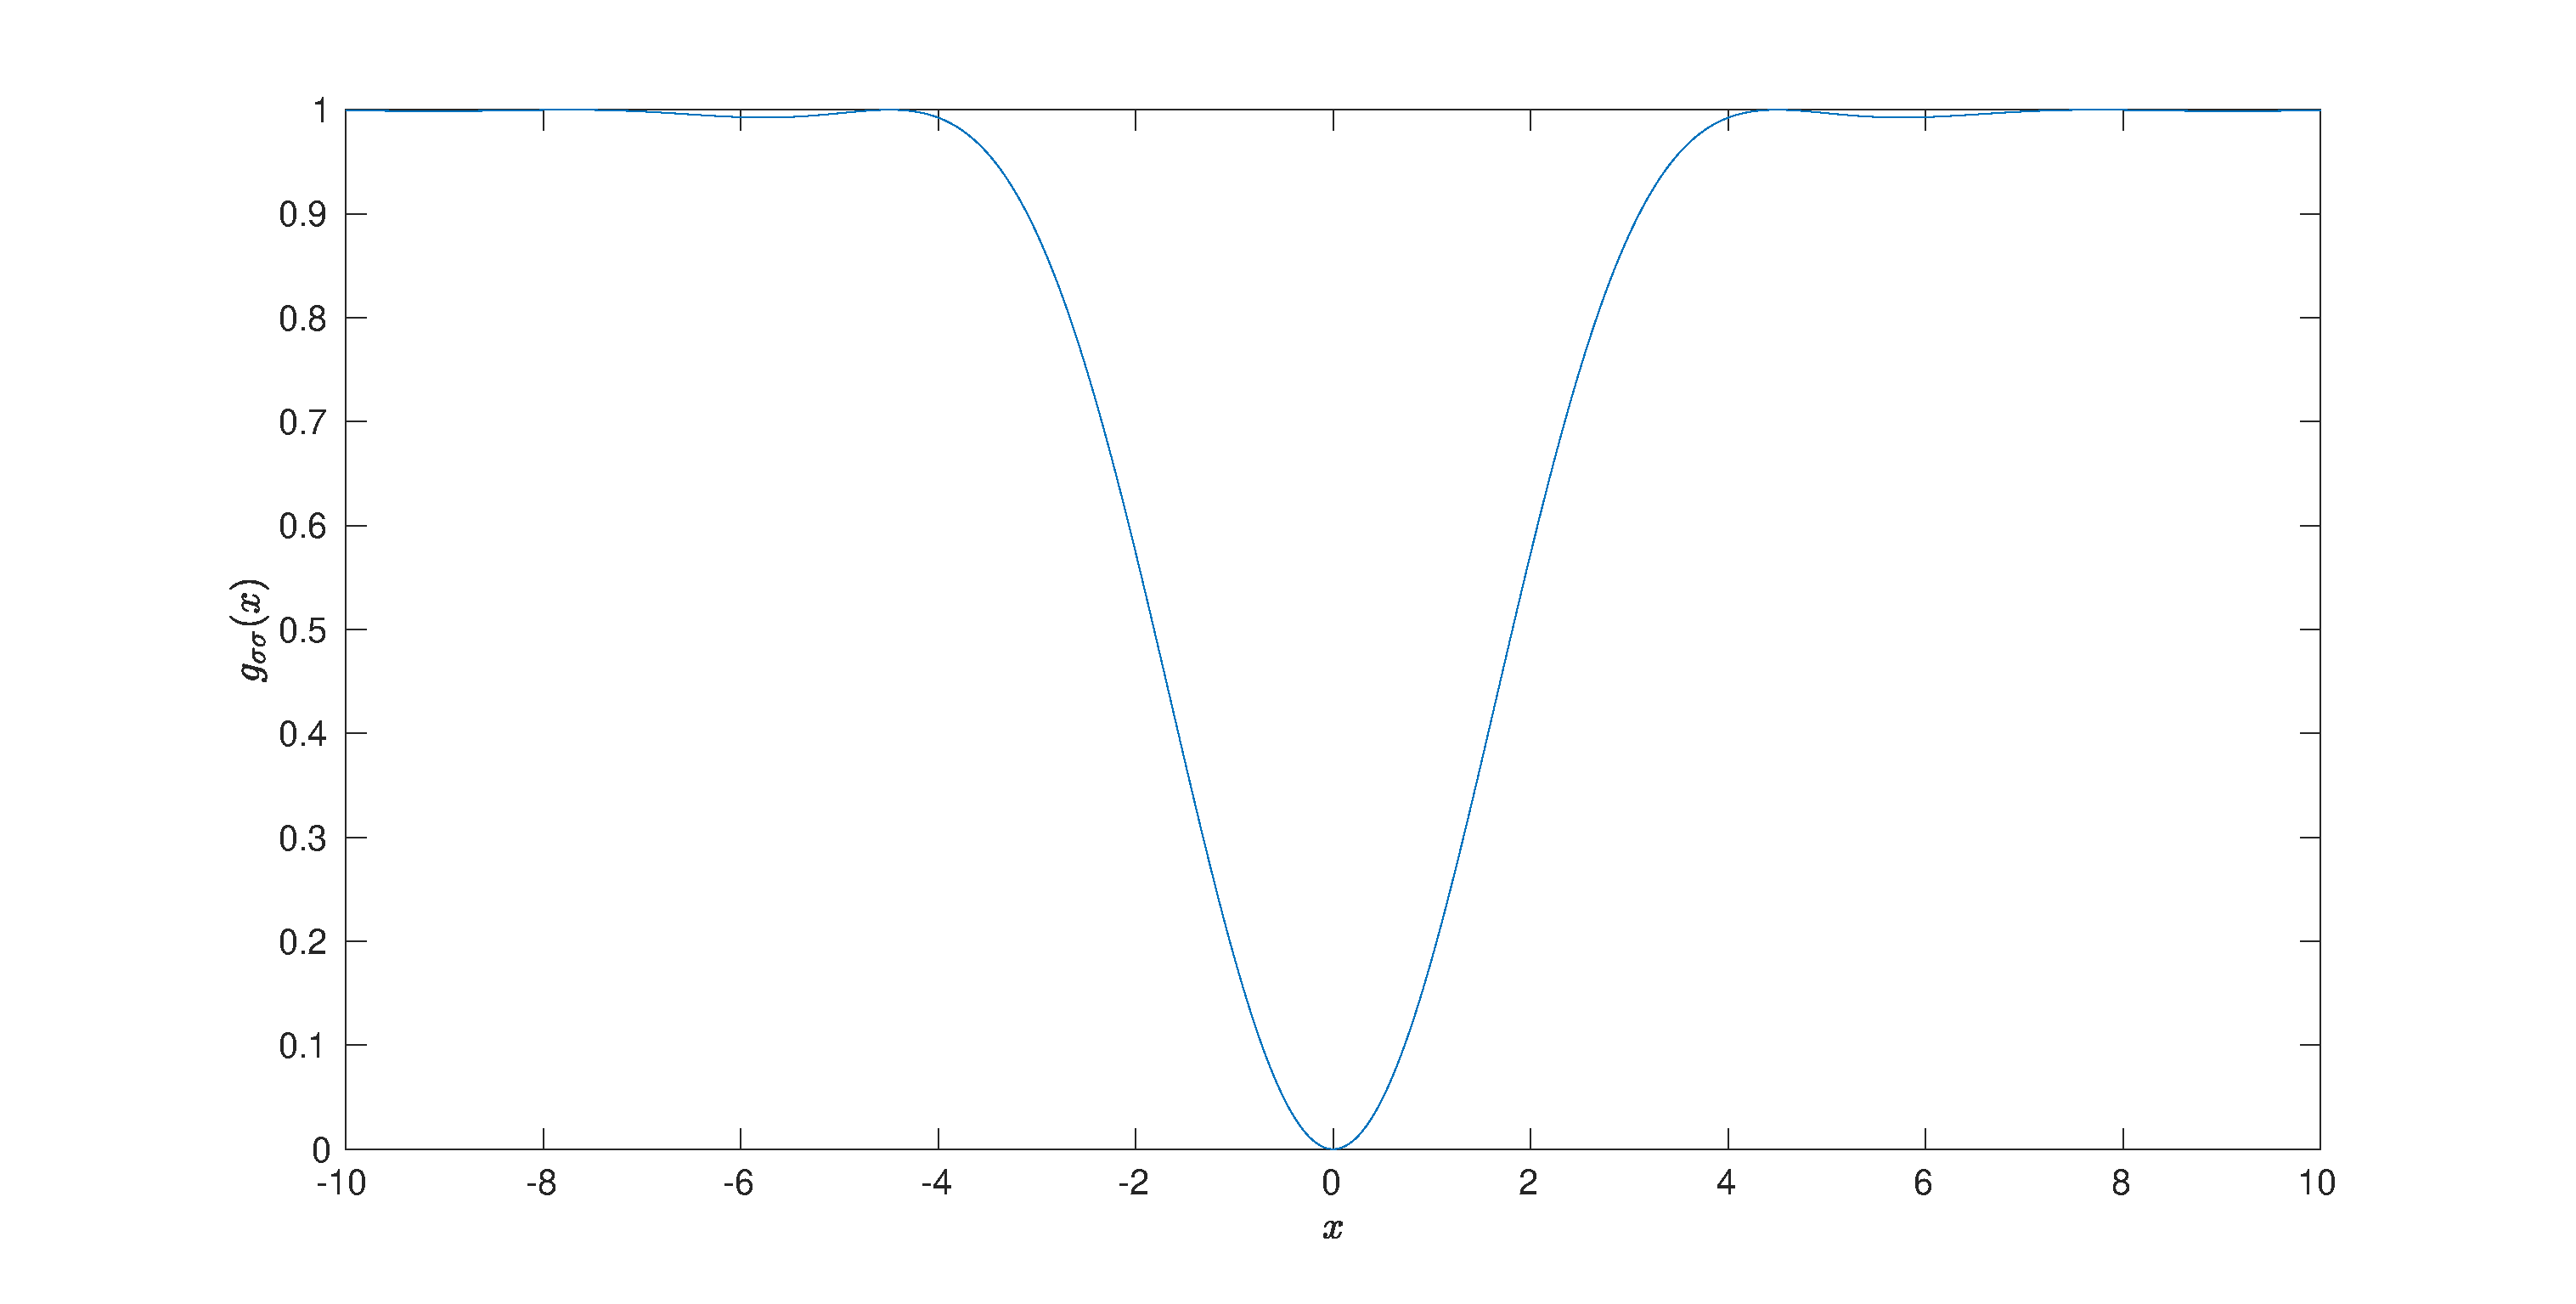
\includegraphics[width=\textwidth]{Density}
\end{figure}
